\documentclass[border=10pt]{standalone}
%%%<
\usepackage{verbatim}
%%%>
\usepackage{pgfplots}
\pgfplotsset{width=7cm,compat=1.8}
\begin{comment}
:Title: Surface plot of a math function
:Tags: 3D;Surfaces;Mathematics;Manual
:Author: Christian Feuersänger
:Slug: surface-plot-math

We would like to plot a function of two variables given by the math expression
exp(-x^2 - y^2) * x.

The code is from the PGFPlots 1.10 manual:
"3.5.4 Computing a Contour Plot of a Math Expression".
\end{comment}
\begin{document}
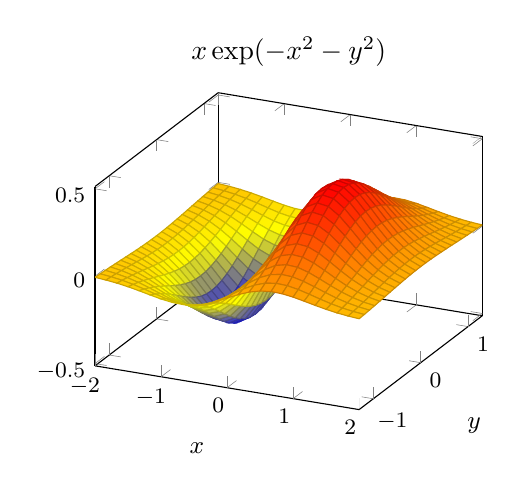
\begin{tikzpicture}
\begin{axis}[
    title={$x \exp(-x^2-y^2)$}, 
    xlabel=$x$, ylabel=$y$,
	small,
]
\addplot3[
	surf,
	domain=-2:2,
	domain y=-1.3:1.3,
] 
	{exp(-x^2-y^2)*x};
\end{axis}
\end{tikzpicture}
\end{document}
